%!TEX root = ../physical-olympics-2.tex
\chapter{静磁场} 


\section{电流与磁场}

\subsection{磁场地位与电流分布}

\begin{itemize}
\item 磁场:\,运动电荷之间的相互作用.\,只有运动电荷才产生磁场,\,磁场也只对运动电荷造成力.

\item 但是运动与静止具有相对性,\,所以磁场是电场的相对论效应.\,即,\,如果认可一个参考系中电荷产生了磁场,\,那么就必须任何换一个参考系以后电荷也以另一种方式产生了相似的物质,\,但是如果变换到相对电荷静止的参考系,\,发现只存在电场,\,这就证明了磁场与电场描述的不过是同一种物质:\,\emph{电磁场}(electromagneto field).

\item 根据相对论的力变换公式:
\[F_x'=F_x-\frac{u}{c^2}\cdot\frac{v_yF_y+v_zF_z}{1-\frac{uv_x}{c^2}}\quad ,\quad F_y'=\frac{F_y}{\gamma (1-\frac{uv_x}{c^2})}\quad ,\quad F_z'=\frac{F_z}{\gamma (1-\frac{uv_x}{c^2})}\]

假设原参考系中只有电场,\,那么无论原参考系中的速度$v_x,\,v_y,\,v_z$如何,\,受力都不取决于速度大小,\,它是:
\[F_x=qE_x\quad ,\quad F_y=qE_y \quad ,\quad  F_z=qE_z\]

代入原式,\,并假设原参考系速度和变换速度相对$c$都是小量,\,故新参考系速度可以使用经典的速度叠加:
\[v_x=v_x'+u\quad ,\quad v_y=v_y' \quad ,\quad v_z=v_z'\]

近似到与$v_x',\,v_y',\,v_z'$一阶相关的领头项:

\[F_x'=qE_x-qv_y'\cdot \frac{uE_y}{c^2}-qv_z'\cdot \frac{uE_z}{c^2}\]
\[F_y'=qE_y+qv_x'\cdot \frac{uE_y}{c^2}\]
\[F_z'=qE_z+qv_x'\cdot \frac{uE_z}{c^2}\]

我们如果假设以下\emph{洛伦兹力}(Lorentz force)公式的成立性:
\[\bs{F}=q(\bs{E}+\bs{v}\times \bs{B})\]

事实上,\,这构成了磁场的严格定义,\,而且具有相对论协变性,\,这一点以后近代物理部分还会加以讨论.\,这个式子即:
\[F_x'=qE_x'+qv_y'B_z'-qv_z'B_y'\]
\[F_y'=qE_y'+qv_z'B_x'-qv_x'B_z'\]
\[F_z'=qE_z'+qv_x'B_y'-qv_y'B_x'\]

对比即知道:
\[B_x'=0\quad ,\quad B_y'=\frac{uE_z}{c^2} \quad ,\quad B_z'=-\frac{uE_x}{c^2}\]

这实际上是:
\[\bs{B}=-\frac{\bs{u}\times \bs{E}}{c^2}\]

如果原参考系是静止点电荷产生的电场,\,现在换参考系以后,\,点电荷做速度为$-\bs{u}$的匀速直线运动而产生以上磁场,\,那么就能推理出,\,如果点电荷以速度$\bs{v}$做匀速直线运动,\,那么它产生的磁场必然为:
\[\bs{B}=\frac{1}{4\pi \varepsilon_0 c^2}\frac{q\bs{v}\times \bs{e}_r}{r^2}\]

这其实就已经是毕奥-萨伐尔定律了,\,只不过历史上它是先通过\emph{奥斯特}(H. C. \O rsted)发现电流的磁效应,\,外加\emph{安培}(A. M. Amp\`ere)等人精妙设计的实验以实验规律给出,\,其形式略有变化,\,见下.\,表面上看推导出的毕奥-萨伐尔定律仅在低速下成立,\,但是麦克斯韦方程的协变性反过来证明了低速下它也是对的.

\item 本章讨论仅限于静磁场,\,即电流分布不随时间改变的磁场,\,上一节告诉我们这就是要求:
\[\nabla \cdot \bs{j}=0\]

\item 电荷运动,\,体电流元,\,面电流元,\,线电流元的等价性:
\[q\bs{v}\sim \bs{j}\ud V \sim \bs{i}\ud S\sim I\ud \bs{l}\]

\end{itemize}

\subsection{毕奥-萨伐尔定律}

\begin{itemize}
\item 电场与磁场的定义:\,任何情况下都是通过洛伦兹力公式:
\[\bs{F}=q(\bs{E}+\bs{v}\times \bs{B})\]

\item 磁场的国际单位:
\[1{\rm T}=10^4{\rm Gs}=1{\rm N/(A\cdot m)}\]

\item 实验规律:\,\emph{毕奥-萨伐尔定律}(Biot-Savart law):
\[\ud \bs{F}_{12}=I_2\ud \bs{l}_2\times \ud \bs{B}_{12}\quad ,\quad \ud \bs{B}_{12}=\frac{\mu_0}{4\pi}\frac{I_1\ud \bs{l}_1\times \bs{e}_{12}}{r^2}\]

虽然是实验规律,\,但之后的理论发展使得其中$\mu_0$不是新的常数,\,它直接被定义为:
\[\mu_0=\frac{1}{\varepsilon_0 c^2}=1.256637062\cdots \times10^{-6}{\rm H/m}\]

称作\emph{真空磁导率}(magnetic permeability of vacuum).
\end{itemize}


\section{两个定律与矢势}

\subsection{磁场环路定律}

\begin{itemize}

\item 磁场环路定律,\,又名安培环路定律:
\[\oint\limits_{\partial S}\bs{B}\cdot \ud \bs{l}=\mu_0 \int\limits_S\bs{j}\cdot \ud \bs{S}\]
\[\nabla\times \bs{B}=\mu_0 \bs{j}\]

\item 
\end{itemize}

\subsection{矢势与磁场高斯定律}

\begin{itemize}

\item 对电流元引入以下矢量场是方便的:
\[\bs{A}=\frac{\mu_0}{4\pi}\frac{\bs{j}\ud V}{r}\]

这是因为计算可得,\,这直接导致了:
\[\bs{B}=\frac{\mu_0}{4\pi}\frac{\bs{j}\ud V\times \bs{e}_r}{r^2}=\nabla\times \bs{A}\]

这个矢量称作\emph{磁矢势}(magnetic vector potential).

\item 由于叠加原理,\,一个电流分布体系的磁矢势和磁场应当为:
\[\bs{A}=\int\limits_V \frac{\mu_0}{4\pi}\frac{\bs{j}\ud V}{r}\quad ,\quad \bs{B}=\int\limits_V \frac{\mu_0}{4\pi}\frac{\bs{j}\ud V\times \bs{e}_r}{r^2}\]

同样地将满足:
\[\bs{B}=\nabla\times \bs{A}\]

\item 以上旋度关系写成积分形式意味着一种计算磁通量的特殊方法:
\[\Phi=\oint\limits_{\partial S} \bs{A}\cdot \ud \bs{l}=\int\limits_S\bs{B}\cdot \ud \bs{S}\]


\item 对于无边界的闭合曲面,\,上式直接证明了磁场高斯定律:
\[\oint\limits_{\partial V}\bs{B}\cdot \ud \bs{S}=0\]
\[\nabla\cdot \bs{B}=0\]

\item 可以设想存在可以像点电荷产生电场那样的方式产生磁场的物质,\,称作\emph{磁单极子`}(magnetic monopole),\,从而可以产生不为零的净\emph{磁荷}(magnetic charge),\,事实证明这样的物质至今都未曾找到,\,从而相伴的磁场形式也仅仅存在与理论中.\,但是,\,总磁荷为零的体系:\,\emph{磁偶极子}(magnetic dipole),\,不仅仅是纯粹的理论模型,\,后面可以发现线圈产生的磁场与磁偶极子是相似的.
\end{itemize}


\section{电流体系}

\subsection{磁偶极子}

\begin{itemize}
\item \emph{磁偶极子}(magnetic dipole)模型一般不指由正负磁单极子构成的体系,\,和电偶极子类似,\,它也来自矢势与磁场计算过程中的多极展开,\,由于需要用到较深的张量知识,\,在此仅仅给出展开的结果:
\[\bs{m}=\frac{1}{2}\int\limits_V \bs{r}\times \bs{j}\ud V\quad ,\quad \bs{A}=\frac{\mu_0}{4\pi}\frac{\bs{m}\times \bs{e}_r}{r^2}\quad ,\quad B_r=\frac{\mu_0}{4\pi}\frac{2m\cos\theta }{r^3}\quad ,\quad B_\theta=\frac{\mu_0}{4\pi}\frac{m\sin\theta }{r^3}\]

其中$\bs{m}$称作\emph{磁矩}(magnetic moment),\,任何情况下这都会是一个电流体系激发的磁场的领头项,\,因为磁单极子不存在,\,类似点电荷产生平方反比的电场那样的磁荷项,\,由于磁高斯定律,\,永远是不可能的.

\item 一个线圈,\,面矢量为$\bs{S}$,\,它的磁矩,\,由于以下积分公式:
\[\bs{S}=\frac{1}{2}\oint\limits_{\partial S}\bs{r}\times \ud \bs{r}\]

可以发现:
\[\bs{m}=\frac{1}{2}\int\limits_V \bs{r}\times I \ud \bs{l}=I\bs{S}\]

如果考虑$I\to \infty,\,S\to 0$的模型,\,就构成了\emph{点磁偶极子}(point dipole).

\item 磁偶极子的磁势能,\,受力与力矩:
\[V=-\bs{m}\cdot \bs{B}\quad ,\quad \bs{F}=\bs{m}\cdot \nabla\bs{B}\quad ,\quad \bs{M}=\bs{m}\times \bs{B}\]

\end{itemize}

\subsection{磁化强度}

\begin{itemize}
\item \emph{磁化强度}(magnetization):
\[\bs{M}=n\bs{m}\]

\item 磁化强度造成的体电流与面电流分布:
\[\bs{j}_M=\nabla\times \bs{M}\quad ,\quad \bs{i}_M=\bs{M}\times \bs{n}\]


\end{itemize}

\subsection{若干对称体系的磁场}

\begin{itemize}
\item 无限长载流直线:
\[\bs{A}=-\frac{\mu_0 I}{2\pi}\ln r\quad ,\quad \bs{B}=\frac{\mu_0 I}{2\pi r}\bs{e}_\varphi\]

\begin{figure}[H]
\centering
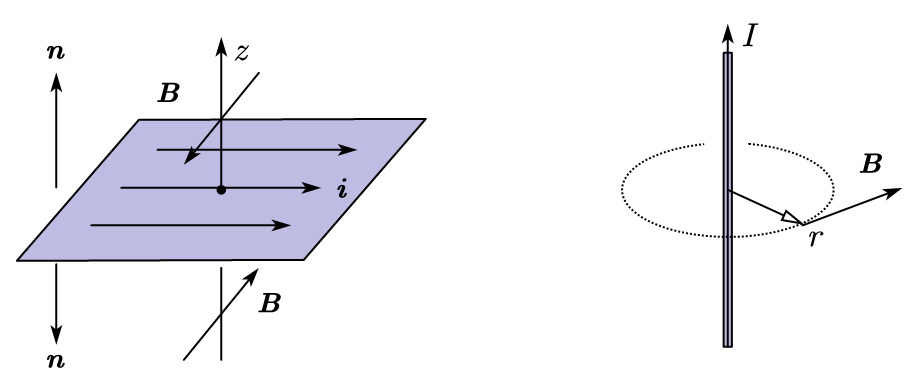
\includegraphics[width=0.7\textwidth]{image/7-4-1.png}
\caption{无限大平面与无限长直线}\label{fig7-4-1}
\end{figure}

\item 无限大载流平面:
\[\bs{B}=\frac{1}{2}\mu_0\bs{i}\times \bs{n}\]

\item 圆环:\,半径为$R$的标准载流线圈轴线上磁场:
\[\bs{B}=\frac{\mu_0IR}{2(R^2+z^2)^{\frac{3}{2}}}\bs{e}_z\]

该处的径向场强可以由磁高斯定理确定:
\[\frac{1}{2}\frac{\ud B_r}{\ud r}+\frac{\ud B_z}{\ud z}=0\quad \Rightarrow \quad B_r\approx -\frac{3\mu_0IRzr}{(R^2+z^2)^{\frac{5}{2}}}\]

\item 无限长密绕螺线管:\,无论其横截面形状,\,总是有:
\[B=\mu_0 i=\mu_0 nI=\frac{\mu_0 NI}{l}\]
\end{itemize}


\npg{-2cm}

\section{磁介质与磁能}

\subsection{微观角度理解磁化}

\begin{itemize}
\item 分子的固有磁矩:\,电子自旋磁矩+电子轨道磁矩.
\item 如果分子具有固有磁矩,\,那么按照热力学规律发生取向磁化:\,磁矩倾向于取与外磁场相同的方向,\,宏观上产生\emph{顺磁性}(paramagnetism).\,类似于电介质的极化,\,微观上顺磁磁化规律可以写作:
\[\bar{\bs{\mu}}=\alpha \bs{B}\]
\item 电子的磁矩与角动量的比称为\emph{旋磁比}(gyromagnetic ratio),\,轨道旋磁比与自旋旋磁比分别为:
\[\gamma_L=-\frac{e}{2m_e}\quad ,\quad \gamma_S=-\frac{e}{m_e}\]

角动量量子化理论告诉我们,\,$z$方向上电子轨道与自旋角动量只能为:
\[L_z=\pm n\hbar \quad ,\quad  S_z=\pm \frac{\hbar}{2}\]

故$z$方向上的磁矩的单位就是著名的\emph{玻尔磁子}(Bohr magneton):
\[\mu_B=\frac{e\hbar}{2m_e}=0.00579{\rm meV/T}\]

事实上由于自旋-轨道耦合,\,分子磁矩可以是玻尔磁子的分数倍.

\item 原子核也有磁矩,\,显然由于质子质量比质子质量大三个量级,\,故根据旋磁比算法,\,其磁矩也小三个量级.\,虽然对分子磁矩和宏观磁化几乎没有贡献,\,但是利用在磁场下形成的各个能级间跃迁吸收发射电磁辐射的原理可以造成\emph{核磁共振}(nuclear magnetic resonance)现象.

\item 如果分子的固有磁矩为零,\,那么在外磁场下会产生一个与外磁场反向的磁矩,\,宏观上造成\emph{抗磁性}(diamagnetism).\,从微观来看似乎与电介质极化的方向相反,\,但是从宏观效果上却与电介质削弱电场的效果相同,\,这是电与磁固有的区别导致的.

\item 抗磁性的微观起源为电子轨道运动的\emph{拉莫尔进动}(Larmor precession).\,由轨道运动产生的力矩,\,角动量,\,磁矩三者关系可得:
\[\bs{M}=\bs{\mu}\times \bs{B}\quad ,\quad  \bs{\mu}=\gamma \bs{L}\quad ,\quad  \frac{\ud}{\ud t}\bs{L}=\bs{M}\]
\[\Rightarrow \quad  \frac{\ud}{\ud t}\bs{L}=-\gamma \bs{B}\times \bs{L}=\frac{e\bs{B}}{2m}\times \bs{L}\]

故在运动学上,\,电子将以以下角速度发生进动:
\[\bs{\Omega}=\frac{e}{2m}\bs{B}\]

电子原来的轨道运动半径如果按照玻尔半径$a_0$估计,\,而角动量量级为$\hbar$,\,那么现在附加的角速度与原来的角速度的比为:
\[\Omega/\omega\sim\frac{ea_0^2}{2\hbar}B\]

故产生的磁矩与原来的玻尔磁子的比值的量级也与之相当,\,得到磁矩的量级为:
\[\bar{\bs{\mu}}\sim-\frac{e^2a_0^2	}{4m}\bs{B}\]

系数便是抗磁性磁化的分子磁化率的量级,\,它一般比顺磁性磁化要小一到两个量级.

\item 有一些金属,\,或者特殊的金属化合物具有独特的\emph{铁磁性}(ferromagnetism),\,微观上它们由介观的包含大量原子的\emph{磁畴}(magnetic domains)构成.\,每一个磁畴由于单元之间的关联已经超过了热力学的涨落而成为了决定性的因素,\,使得所有电子的自旋几乎都严格指向同一个方向,\,磁化达到饱和.\,而材料的磁化过程其实是不同的磁畴在外磁场下的转向.\,它的磁化率将远远大于简单的顺磁和抗磁磁化.\,而且体现出非线性和历史相关性.


\end{itemize}

\subsection{宏观角度理解磁化}

\begin{itemize}
\item 出于$\bs{B}$和$\bs{M}$的旋度分别为总电流密度和磁化电流密度,\,引入\emph{磁场强度}(magnetic field strength)以区别于以往一贯描述磁场的$\bs{B}$,\,一般可区别称作\emph{磁通密度}(magnetic flux density):
\[\bs{H}=\frac{\bs{B}}{\mu_0}-\bs{M}\]

这样这个矢量的旋度就只取决于外电流:
\[\nabla\times \bs{H}=\bs{j}_f\]

\item 在顺磁或铁磁的柱状介质外绕制密绕螺线管,\,那么没有介质时其磁通密度为:
\[B_0=\mu_0 i\]

那么,\,由于此时加入介质时磁化电流不影响$\bs{H}$的计算,\,故磁场强度为:
\[H=\frac{B_0}{\mu_0}=i\]

但是磁化电流的存在将产生一个与原磁场同向的附加磁场,\,使得介质内部的磁场变大,\,那么定义此时磁场与原磁场的比值为\emph{相对磁导率}(relative magnetic permeability):
\[B/B_0=\mu_r\]

那么把绝对磁导率定义为$\mu=\mu_r\mu_0$,\,就有以下关系式:
\[B=\mu H=\mu i\]

\[M=(\mu_r-1)H=\chi_m H\]

其中$\chi_m$就是宏观的\emph{磁化率}(magnetic susceptibility).\,对于抗磁性物质,\,其值是小于零的.


\end{itemize}

\subsection{磁场能量}

磁场体系的能量的计算方法可以证明可以有用电流与矢势和用能量密度两种计算方法:
\[I=\frac{1}{2}\int \bs{j}\cdot\bs{A}\ud V=\int \frac{1}{2\mu_0}	\bs{B}^2\ud V\]

同样地,\,两个体系同时存在时,\,体系将产生自能与相互作用能.\,如两个电感元件如果之间存在互感,\,那么其总能量应当为:
\[E=\frac{1}{2}L_1I_1^2+\frac{1}{2}L_2I_2^2+ MI_1I_2\]

如果存在介质,\,其能量密度需要加上磁化带来的能量,\,能量密度变为:
\[w=\frac{1}{2\mu}	\bs{B}^2=\frac{1}{2}\mu \bs{H}^2 =\frac{1}{2}	\bs{B}\cdot \bs{H}\]

%\section{超导简介}
